\begin{frame}
  \subsection{Overflateintegral}
  \frametitle{Overflateintegral}
  \centerline{%
    \only<1>{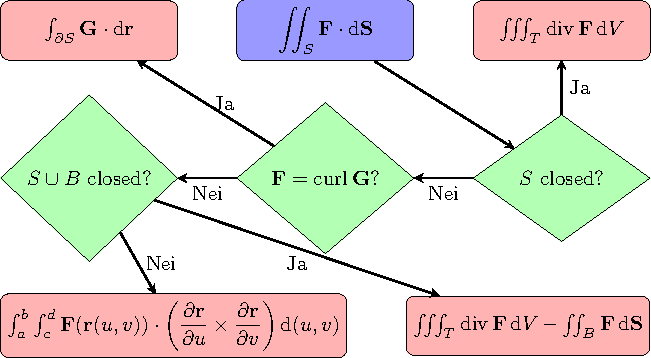
\includegraphics{../img/flytskjema-overflateintegral}}
    \only<2>{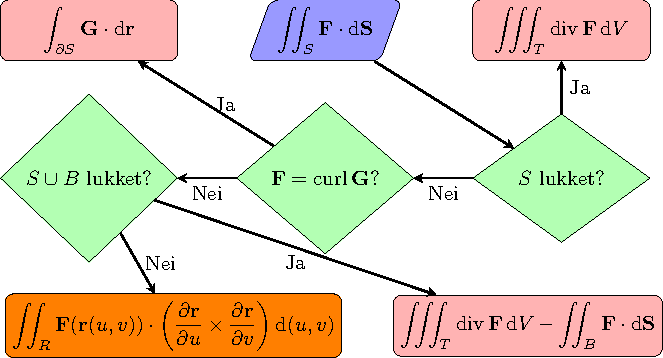
\includegraphics{../img/flytskjema-overflateintegral-0}}
  }
  $S$ er en parametrisert flate $S \colon \rr(u,v), (u,v) \in R \subseteq \R^2$ med rand $\partial S$. \\
  $T$ er volumet med overflate $S$. $B$ er en tiltenkt flate (lokk til $S$).
\end{frame}

\begin{frame}
  \begin{enumerate}
    \item Tegn integrasjonsområdet og bestem integrasjonsgrensene
    \item Bestem parametriseringen $\rr(u,v) \colon (u,v) \in R$ og
      $
        \diffp{\rr}{u}\times\diffp{\rr}{v}
      $.
    \item Dersom $\F(x,y)$ er et vektorfelt blir fluksen ut av oveflaten
      \begin{align*}
        \iint_S \F \cdot \dS & =
        \iint_R \F(\rr(u,v)) \cdot \left( \diffp{\rr}{u}\times\diffp{\rr}{v} \right)\dd(x,y)\,.
      \intertext{Dersom $z = g(x,y)$ så er $\rr(x,y) = (x,y,g(x,y))$, $(x,y) \in R$ og}
        \iint_S \F \cdot \dS & =
        \iint_R\,(F_1, F_2, F_3) \cdot (-g_x,-g_y,1) \dd(x,y).
      \end{align*}
    \item Dersom $g(x,y)$ er et skalarfelt er overflateintegralet gitt som
      \begin{align*}
        A & =
        \iint_S\,\norm*{\diffp{\rr}{u}\times\diffp{\rr}{v}}\dd(u,v)\,,
      \intertext{I spesialtilfelle $z = g(x,y)$ er $\rr(u,v) = (x,y,g(x,y))$ og}
      %
        A & =
        \iint_T \sqrt{\left( \diffp{f}{x} \right)^2+\left( \diffp{f}{y} \right)^2+1} \dd(x,y).
      \end{align*}
  \end{enumerate}
\end{frame}

\begin{frame}
  \begin{oppgave}{V2015, Oppgave 5b}
    La $g(x,y) = 1+\frac{y^2}{2x}$ være definert på $g\colon D \to \R$ hvor
    $D = \{(x,y) \in \R^2 \mid 1 \leq x \leq 9, -3 \sqrt{x} \leq y \leq 3 \sqrt{x}\}$
    \\ bestem arealet av flaten $S = \{(x,y,z)\in \R^3 \mid z = g(z,y), (x,y) \in D\}$.
  \end{oppgave}
  \begin{enumerate}
    \item Tegn integrasjonsområdet og bestem integrasjonsgrensene
  \end{enumerate}
  \begin{minipage}[b]{0.45\textwidth}\centering
    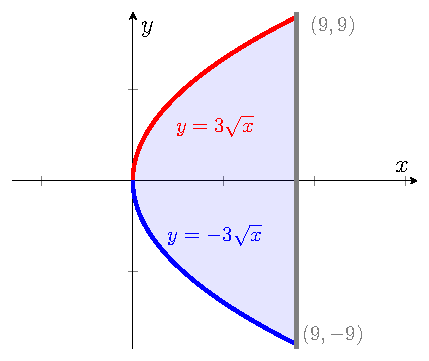
\includegraphics{../img/overflateintegral-2015V}
  \end{minipage}\hfill
  \begin{minipage}[b]{0.45\textwidth}\centering\vspace*{-3cm}
  \begin{align*}
    \begin{split}
    1 \leq & x \leq 9 \\
    -3 \sqrt{x} \leq & y \leq 3 \sqrt{x}
  \end{split} \\ \ & \Downarrow \ \\
   \iint_D \dd(x,y) & = \int_1^{9} \int_{-3\sqrt{x}}^{3\sqrt{x}}\dy \dx
  \end{align*}
  \vspace{1cm}
  \phantom{a//a//a//a//a//a//a//a//a//a//a}
  \end{minipage}
\end{frame}

\begin{frame}
  \begin{oppgave}{V2015, Oppgave 5b}
    La $g(x,y) = 1+\frac{y^2}{2x}$ være definert på $g\colon D \to \R$ hvor
    $D = \{(x,y) \in \R^2 \mid 1 \leq x \leq 9, -3 \sqrt{x} \leq y \leq 3 \sqrt{x}\}$
    bestem arealet av flaten $S = \{(x,y,z)\in \R^3 \mid z = g(z,y), (x,y) \in D\}$.
  \end{oppgave}
  \begin{enumerate}
      \stepcounter{enumi}
    \item Bestem parametriseringen $\rr(u,v) \colon (u,v) \in R$ og
      $
      \diffp{\rr}{u}\times\diffp{\rr}{v}
      $.
  \end{enumerate}
      Parametriseringen vil være: $\mathbf{r}(x, y)=(x, y, g(x,y))$, $(x,y)\in D$  Slik at $\frac{\partial
        \mathbf{r}}{\partial x}=(1, 0, g_x(x,y))$, og $\frac{\partial
        \mathbf{r}}{\partial y}=(0, 1, g_y(x,y))$.  Så,
      \begin{equation}
        \diffp{\rr}{x}\times\diffp{\rr}{y}
        = \begin{vmatrix}
          \I & \J & \K \\
          1 & 0 & \diffp{g}{x} \\[0.2cm]
          0 & 1 & \diffp{g}{y}
        \end{vmatrix}
        = \left( -\diffp{g}{x}, -\diffp{g}{y}, 1 \right)
      \end{equation}
  \end{frame}

\begin{frame}
  \begin{oppgave}{V2015, Oppgave 5b}
    La $g(x,y) = 1+\frac{y^2}{2x}$ være definert på $g\colon D \to \R$ hvor
    $D = \{(x,y) \in \R^2 \mid 1 \leq x \leq 9, -3 \sqrt{x} \leq y \leq 3 \sqrt{x}\}$
    bestem arealet av flaten $S = \{(x,y,z)\in \R^3 \mid z = g(z,y), (x,y) \in D\}$.
  \end{oppgave}
  \begin{enumerate}
      \stepcounter{enumi}
      \stepcounter{enumi}
    \item Dersom $g(x,y)$ er et skalarfelt er overflateintegralet gitt som
  \end{enumerate}
      \begin{align*}
        A = \iint\limits_S \dSS
        & = \iint\limits_D \only<1-2>{\norm*{  \only<1>{\diffp{\rr}{x}\times\diffp{\rr}{y}}  \only<2>{\left(-\diffp{g}{y}, -\diffp{g}{y}, 1\right)}}} \only<3->{\sqrt{1 + \left( \diffp{g}{x} \right)^2+\left( \diffp{g}{y} \right)^2}} \dd (x,y) \only<4->{\\
        & = \int_1^9 \int_{-3\sqrt{x}}^{3\sqrt{x}}\sqrt{\only<4>{1 + \left( -\frac{y^2}{2x^2} \right)^2 + \left( \frac{y}{x} \right)^2}\only<5>{\textcolor{red}{1}^2 + 2 \cdot \textcolor{red}{1} \cdot \textcolor{blue}{  \frac{y^2}{2x^2}} + \left( \textcolor{blue}{\frac{y^2}{2x^2}} \right)^2}\only<6>{\left( \textcolor{red}{1} + \textcolor{blue}{\frac{y^2}{2x^2}} \right)^2}\only<7->{\left( 1 + \frac{y^2}{2x^2} \right)^2}}\dy\dx}
          \only<5>{\\
          [\textcolor{red}{a}^2 + 2\cdot\textcolor{red}{a}\cdot\textcolor{blue}{b} + \textcolor{blue}{b}^2 & = (\textcolor{red}{a} + \textcolor{blue}{b})^2]}
                                                                                                             \only<6-7>{\\& = \int_1^9 \only<6>{\left[ y + \frac{y^3}{6x^2} \right]_{-3\sqrt{x}}^{3\sqrt{x}}}\only<7>{6 \sqrt{x} + \frac{9}{\sqrt{x}}}\dx}
                                                                                                                          \only<8>{\\& = \left[ 4x^{3/2} + 18x^{1/2} \right]_1^9}
                                                                                                                          \only<9>{\\& = 140}
      \end{align*}
    \only<3>{%
    \begin{intuisjon}
      Fra Analyse I husker vi at lengden av en funksjon var gitt som
      %
      \begin{equation*}
        L = \int_a^b \sqrt{1 + \left( \diffp{f}{x} \right)^2} \dx
      \end{equation*}
      %
      Altså ser vi at et overflateintegral kan betraktes som et to-dimensjonalt
      buelengdeintegral dersom $z = g(x,y)$.
    \end{intuisjon}}
\end{frame}


%%% Local Variables:
%%% mode: latex
%%% TeX-master: "main"
%%% End:
